\chapter{Methodology}

\label{chapter:methodology}

\begin{figure}[h]
    \centering
    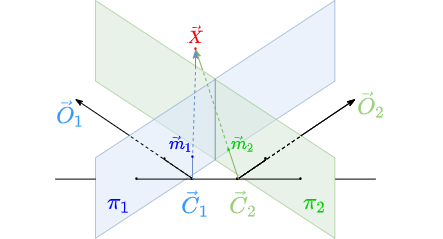
\includegraphics[width=.8\textwidth]{graphics/td90deg.png}
    \caption{The proposed approach model}
    \label{fig:td90deg}
\end{figure}

The main task of this thesis is to create a compact obstacle avoidance system such that it can be mounted on MAVs with size and weight restrictions.
There are related works of a monocular stereovision using SfM or Optical flow algorithms. 
Also, there are some stereovision approaches with standard stereo cameras as on \autoref{fig:stereo_ex}.
The method that combines mono and stereo camera approaches is presented further.

The problem solution can be divided into several steps. 
Firstly, it is necessary to make a math model of a solution and describe its behaviour. 
Secondly, choose hardware parts - cameras and suitable lenses and calibrate each separate camera. 
Thirdly, make a computer-aided design (CAD) model of the cameras' holder, print, and calibrate it.
Fourthly, implement a Robotic operating system (ROS) driver for a proposed device. 
This driver collects images from both cameras with the same timestamp and publishes them together.
Then detect features on both images, find and filter correspondences.
The last step is to compute the distance to visible objects in the cameras' overlapping zone.

As far as the stereo pair is calibrated, the 3D pose estimation depends on a stereo pair calibration, cameras' calibration, key point extractor and matcher.
As a result, extracted features can be used in an SfM algorithm to correct a relative drone pose between $t_0$ and $t_1$ on \autoref{fig:intro_general}.
Estimating distances to objects can be used in a feedback loop inside the system to correct path planning, considering the obstacles found.

This chapter describes a general maths model of a solution and all algorithms used in a process: for camera calibration, stereo pair calibration points' pose obtaining and error measurements.

\section{Model description}

On the \autoref{fig:td90deg}: there are two cameras with centers at $C_1$ and $C_2$ with a known static translation $\vec{t}_{21}$ and rotation $\mat{R}_{21}$, where $\mat{R}_{21}$ corresponds to Euler angle $90^\circ$ rotation in the epipolar plane (\autoref{fig:epipolar_std}, plane $\sigma$).
Both cameras' intrinsic parameters are known, and images are synchronized in time; the FOV of both cameras have an intersecting zone.
Let images from cameras with centers at $C_1$ and $C_2$ be \textit{im1} and \textit{im2} respectively.
In the overlapping zone, there are two interesting points detected and matched as images of a same 3D point $\vec{X}$: $\vec{m}_1$ on \textit{im1} and $\vec{m}_2$ on \textit{im2}.
The 3D pose of a point $\vec{X}$ in world measurement units is obtain from known vectors $\vec{X} - \vec{C}_1$, $\vec{X} - \vec{C}_2$ and $\vec{t}_{21}$. 

The described method assumes that each camera is calibrated, and the stereo pair is also calibrated - both $t_{21}$ and $R_{21}$ are known.

\section{Single camera calibration}
\label{sec:meth_calib}
\begin{figure}[h]
    \begin{subfigure}[b]{0.45\textwidth}
      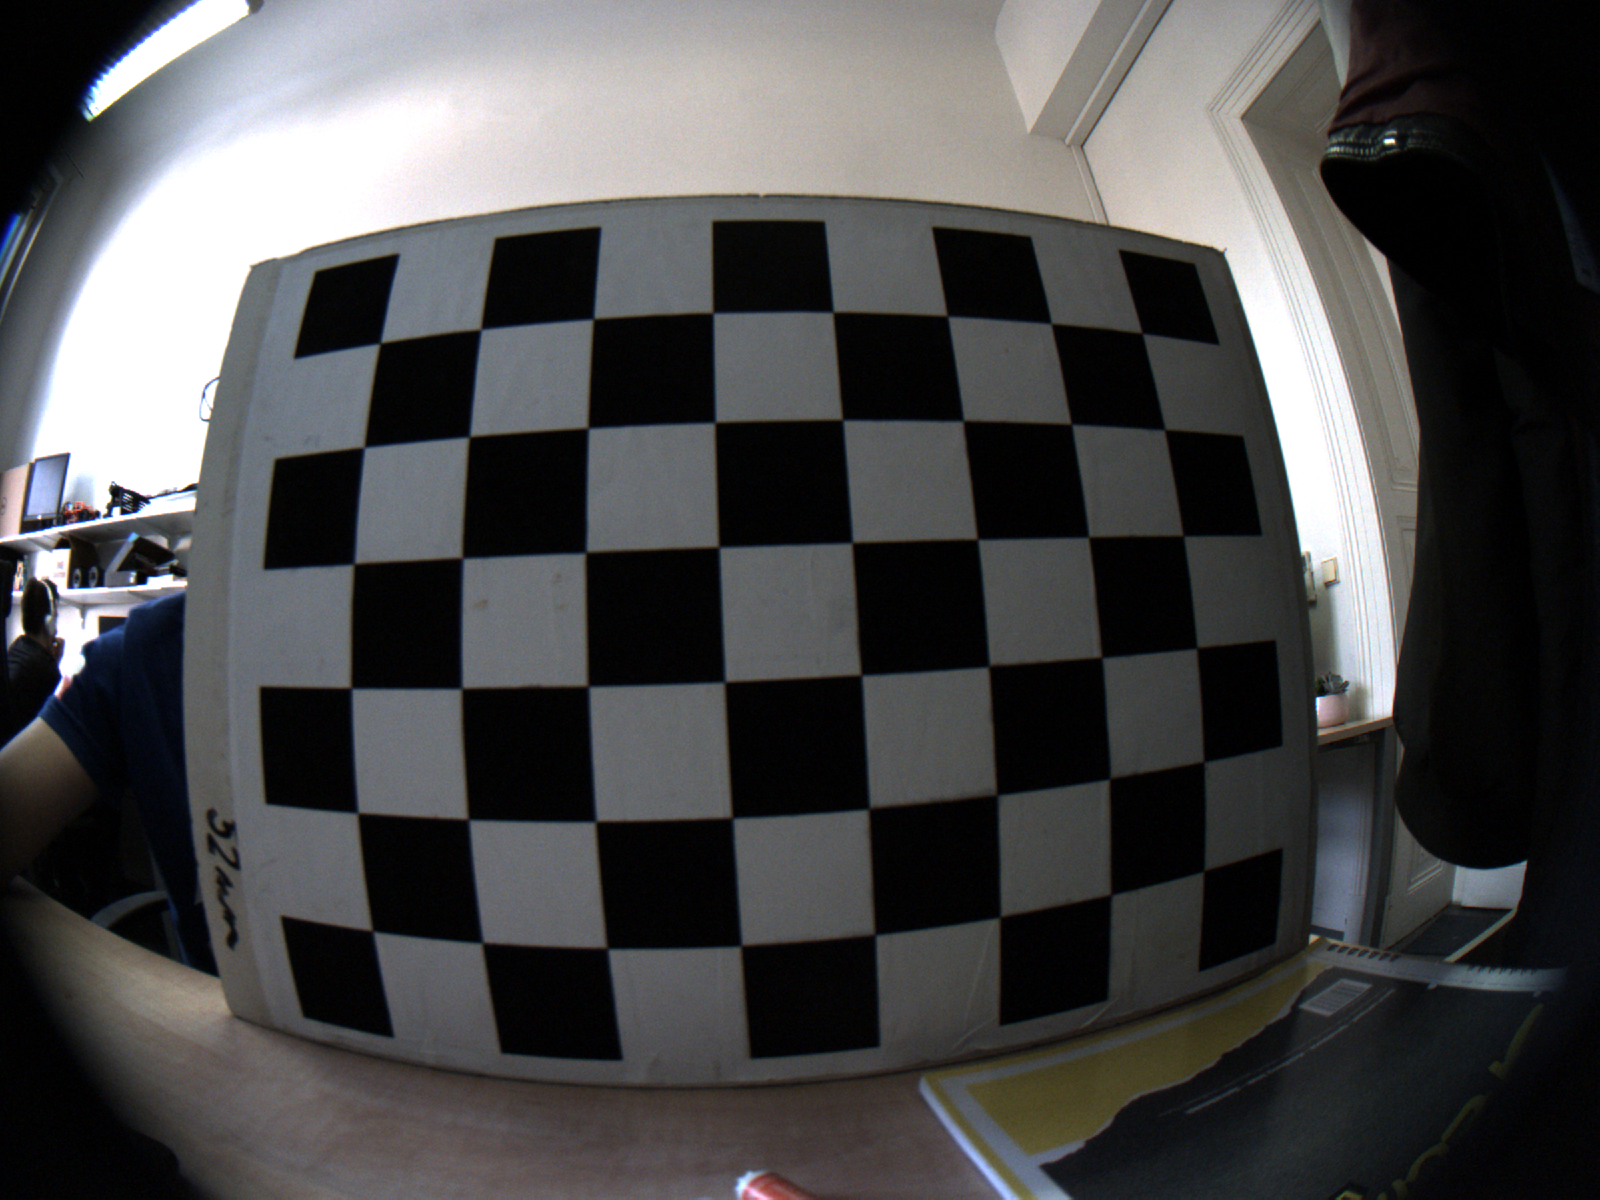
\includegraphics[width=\textwidth]{graphics/chessboard_img.png}
      \caption{Original image with radial distortion.}
      \label{fig:chb1}
    \end{subfigure}
    \hfill
    \begin{subfigure}[b]{0.45\textwidth}
      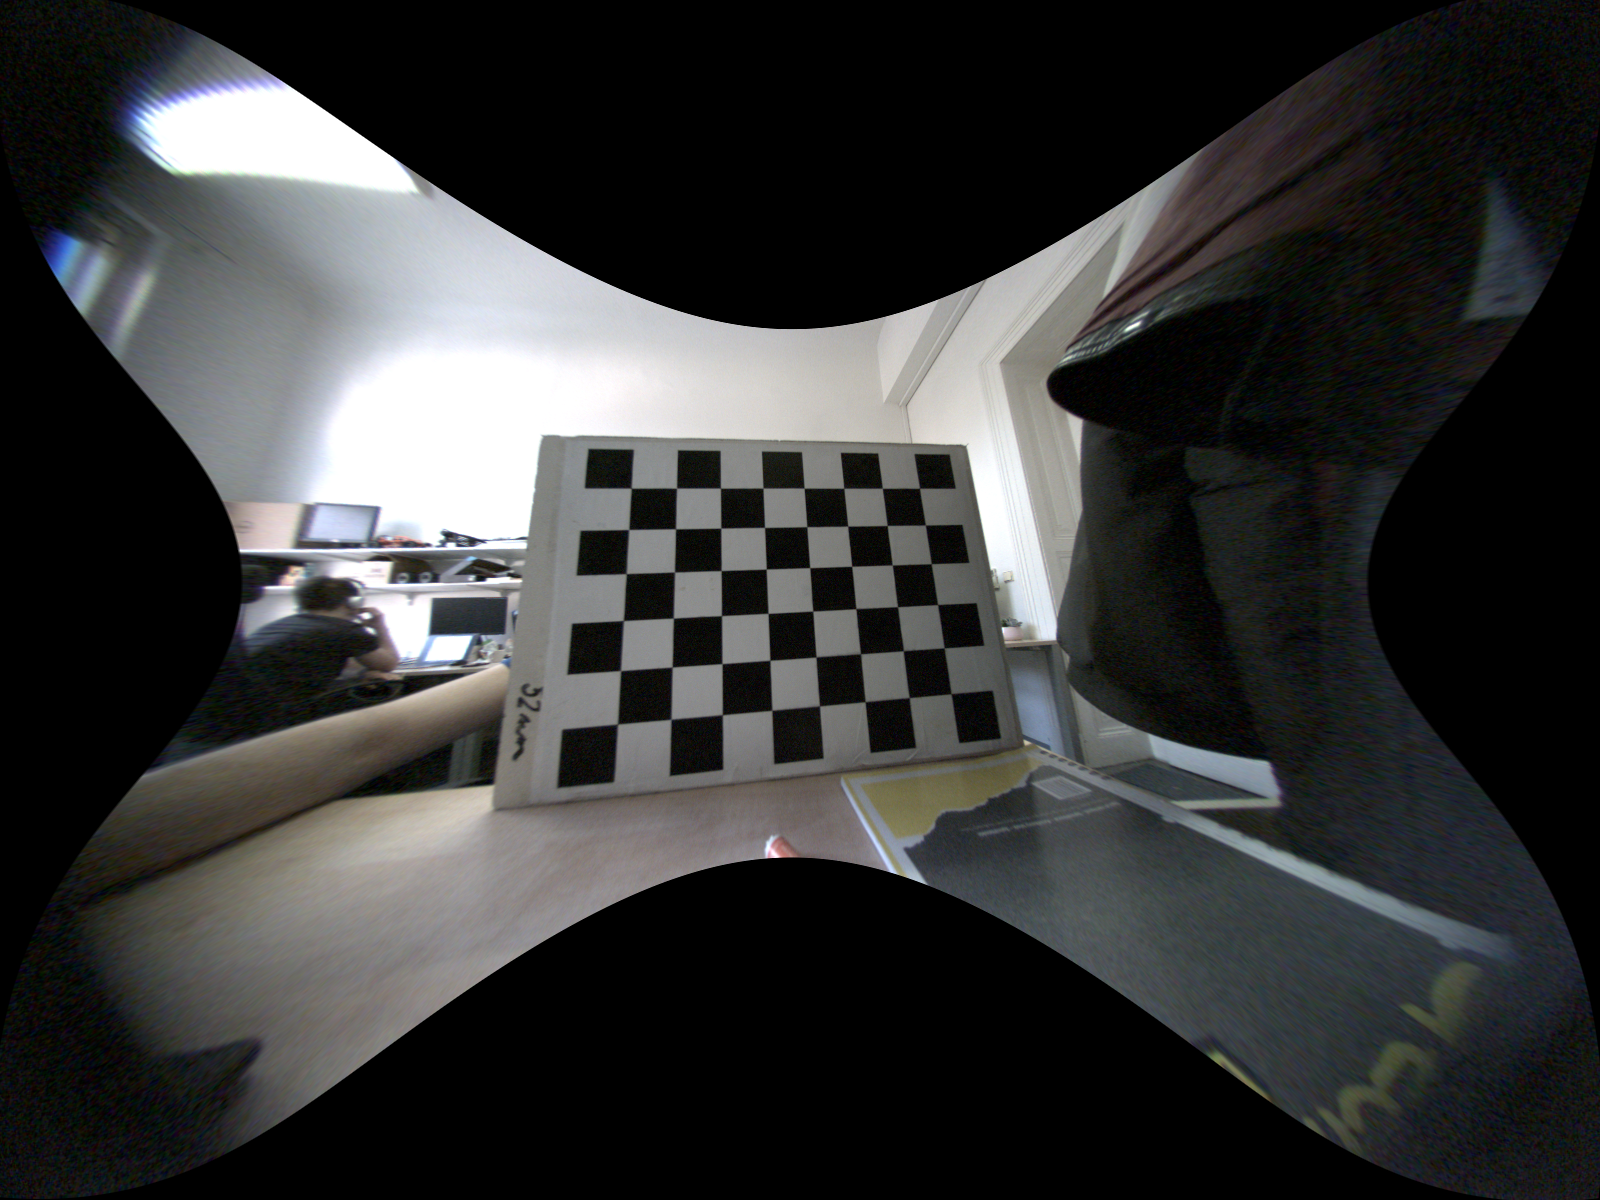
\includegraphics[width=\textwidth]{graphics/chessboard_img_rect.png}
      \caption{Undistorted image with no distortion.}
      \label{fig:chb2}
    \end{subfigure}
    \caption{Camera image before and after the calibration}
    \label{fig:chb}
\end{figure}

Camera calibration - is a process of computing the camera calibration matrix $\mat{K}$ (see \eqref{eq:kmat}).
Usually, it is done with some pattern with predefined parameters, like a chessboard or more advanced markers (ChArUco and ArUco \cite{aruco} etc).

The camera calibration is necessary for geometrical image correction, distortion elimination, obtaining metric information and further distances estimation (\autoref{fig:chb}). 
It is used in most maths for image processing and stereovision, for example, \eqref{eq:PKRt}, \eqref{eq:F}

In the real world, lenses have distortion (see \autoref{fig:chb1}), to compensate that distortion a polynomial model is typically used with coefficients $k_1 ... k_6$ for radial distortion and $p_1, p_2$ for tangential distortion.

\paragraph{The minimal problem for camera calibration.} 
It is the problem of obtaining a projection matrix $\mat{P}$ given $k=6$ correspondences of 3D scene points and 2D image points $\{(\vec{X}_i, \vec{m}_i)\}_{i=1}^k$.
Let the projection matrix $\mat{P}$ be 
\begin{equation}
    \label{eq:p_calib}
    \mat{P} = \begin{bmatrix}
        q_1^\top & q_{14} \\
        q_2^\top & q_{24} \\
        q_3^\top & q_{34} \\
    \end{bmatrix},    
\end{equation}
then the equation \eqref{eq:proj_min} can be expand to
\begin{equation}
    \lambda_i u_i = q_1^\top \vec{X}_i + q_{14}, \;\;\;
    \lambda_i v_i = q_2^\top \vec{X}_i + q_{24}, \;\;\;
    \lambda_i = q_3^\top \vec{X}_i + q_{34}, \;\;\;
\end{equation}
where $\vec{m}_i = \begin{bmatrix} u_i \\ v_i \end{bmatrix}$, $ \lambda \in \mathbb{R}$, $\lambda \neq 0$, $i = 1, 2 ... k$, $k = 6$.
After elimination of $\lambda_i$
\begin{equation}
    (q_3^\top \vec{X}_i + q_{34})u_i = q_1^\top \vec{X}_i + q_{14},
\end{equation}
\begin{equation}
    (q_3^\top \vec{X}_i + q_{34})v_i = q_2^\top \vec{X}_i + q_{24},
\end{equation}
then
\begin{equation}
    \mat{A} \vec{q} = \begin{bmatrix}
        \vec{X}_1^\top & 1 & \vec{0}^\top & 0 & -u_1 \vec{X}_1^\top & -u1 \\
        \vec{0}^\top & 0 & \vec{X}_1^\top & 1 & -v_1 \vec{X}_1^\top & -v_1 \\ 
        \vdots & \vdots & \vdots & \vdots & \vdots & \vdots \\
        \vec{X}_k^\top & 1 & \vec{0}^\top & 0 & -u_k \vec{X}_k^\top & -uk \\
        \vec{0}^\top & 0 & \vec{X}_k^\top & 1 & -v_k \vec{X}_k^\top & -v_k \\ 
    \end{bmatrix} \cdot \begin{bmatrix}
        q_1 \\ q_{14} \\ q_2 \\ q_{24} \\ q_3 \\ q_{34}
    \end{bmatrix} = 0,
\end{equation}
so for $k=6$, $\mat{A} \in \mathbb{R}^{12, 12}$, $\vec{q} \in \mathbb{R}^{12}$. If $\mat{A}$ has rank 12, there is no non-trivial null space for $\mat(A)$.

It can be solved by so-called \textit{Jack-Knife estimation}: iterate through all rows of the matrix $\mat{A}$, $i = 1..12$, let $\mat{A}_i$ be the matrix $\mat{A}$ without $i$-th row.
Then if the right null-space of $\mat{A}_i$ is not empty, matrix $\mat{P}$ from the vector $\vec{q}$ (see \eqref{eq:p_calib}) can be decompesed to $\mat{K}_i$ $\mat{R}_i$ and $\vec{t}_i$.
Minimisation of the reprojection error from \autoref{sec:error_reprojection} for $i = 1..12$ then can be used to find the correct $\mat{P}$.

% \begin{equation}
%     \lambda 
%     \begin{bmatrix} 
%     \vec{m} \\ 1 \end{bmatrix} = \pmb{\mathsf{P}} \begin{bmatrix} \vec{X} \\ 1
%     \end{bmatrix},
% \end{equation}

\paragraph{Distortion correction.}
After matrix $\mat{P}$ was obtained, distortion vector can be found as well.
The equation \eqref{eq:projection} can be rewritten as
\begin{equation}
    \label{eq:dist_start}
    \lambda \begin{bmatrix} 
        u \\ v \\ 1 \end{bmatrix} = \pmb{\mathsf{K}} [\pmb{\mathsf{R}} | \vec{t}] \begin{bmatrix} x \\ y \\ z \\ 1
    \end{bmatrix}.
\end{equation}
Let us now redefine this equation to consider the distortion. A 3D point in the camera frame is 
\begin{equation}
    \label{eq:dist_2}
    \begin{bmatrix} x_c \\ y_c \\ z_c \end{bmatrix}
     = [\pmb{\mathsf{R}} | \vec{t}] \begin{bmatrix} x \\ y \\ z \\ 1
    \end{bmatrix}.
\end{equation}
The distortion model is defined as 
\begin{equation}
    \label{eq:dist_3}
    x'' = \frac{x_c}{z_c} \frac{1 + k_1r^2 + k_2r^4 + k_3r^6}{1 + k_4r^2 + k_5r^4 + k_6r^6} + p_1(r + 2x') + 2p_2\frac{x_c y_c}{z^2_c},
\end{equation}
\begin{equation}
    \label{eq:dist_4}
    y'' = \frac{y_c}{z_c} \frac{1 + k_1r^2 + k_2r^4 + k_3r^6}{1 + k_4r^2 + k_5r^4 + k_6r^6} + 2p_1(\frac{x_c y_c}{z_c^2}) + p_2(r + 2y'),
\end{equation}
where $x' = (\frac{x_c}{z_c})^2$; $y' = (\frac{y_c}{z_c})^2$; $r = x' + y'$. Then the undistorted point will be
\begin{equation}
    \label{eq:dist_end}
    \begin{bmatrix} u \\ v \\ 1 \end{bmatrix} = \pmb{\mathsf{K}} \begin{bmatrix} x'' \\ y'' \\ 1 \end{bmatrix}.
\end{equation}

Considering \eqref{eq:kmat}, the image of a point $X$ seen through the calibrated camera with a projection matrix $\mat{P}$ is obtained using eqs. \eqref{eq:dist_start} to \eqref{eq:dist_end}. 
Firstly, the point is projected to an abstract projection plane (\eqref{eq:dist_2}), then undistorted (\eqref{eq:dist_3}, \eqref{eq:dist_4}) and finally transformed from the metric system of abstract projection plane to the image coordinate system (\eqref{eq:dist_end}).

\section{General multicamera calibration}
\label{sec:stereocalib}

\begin{figure}[h]
    \centering
    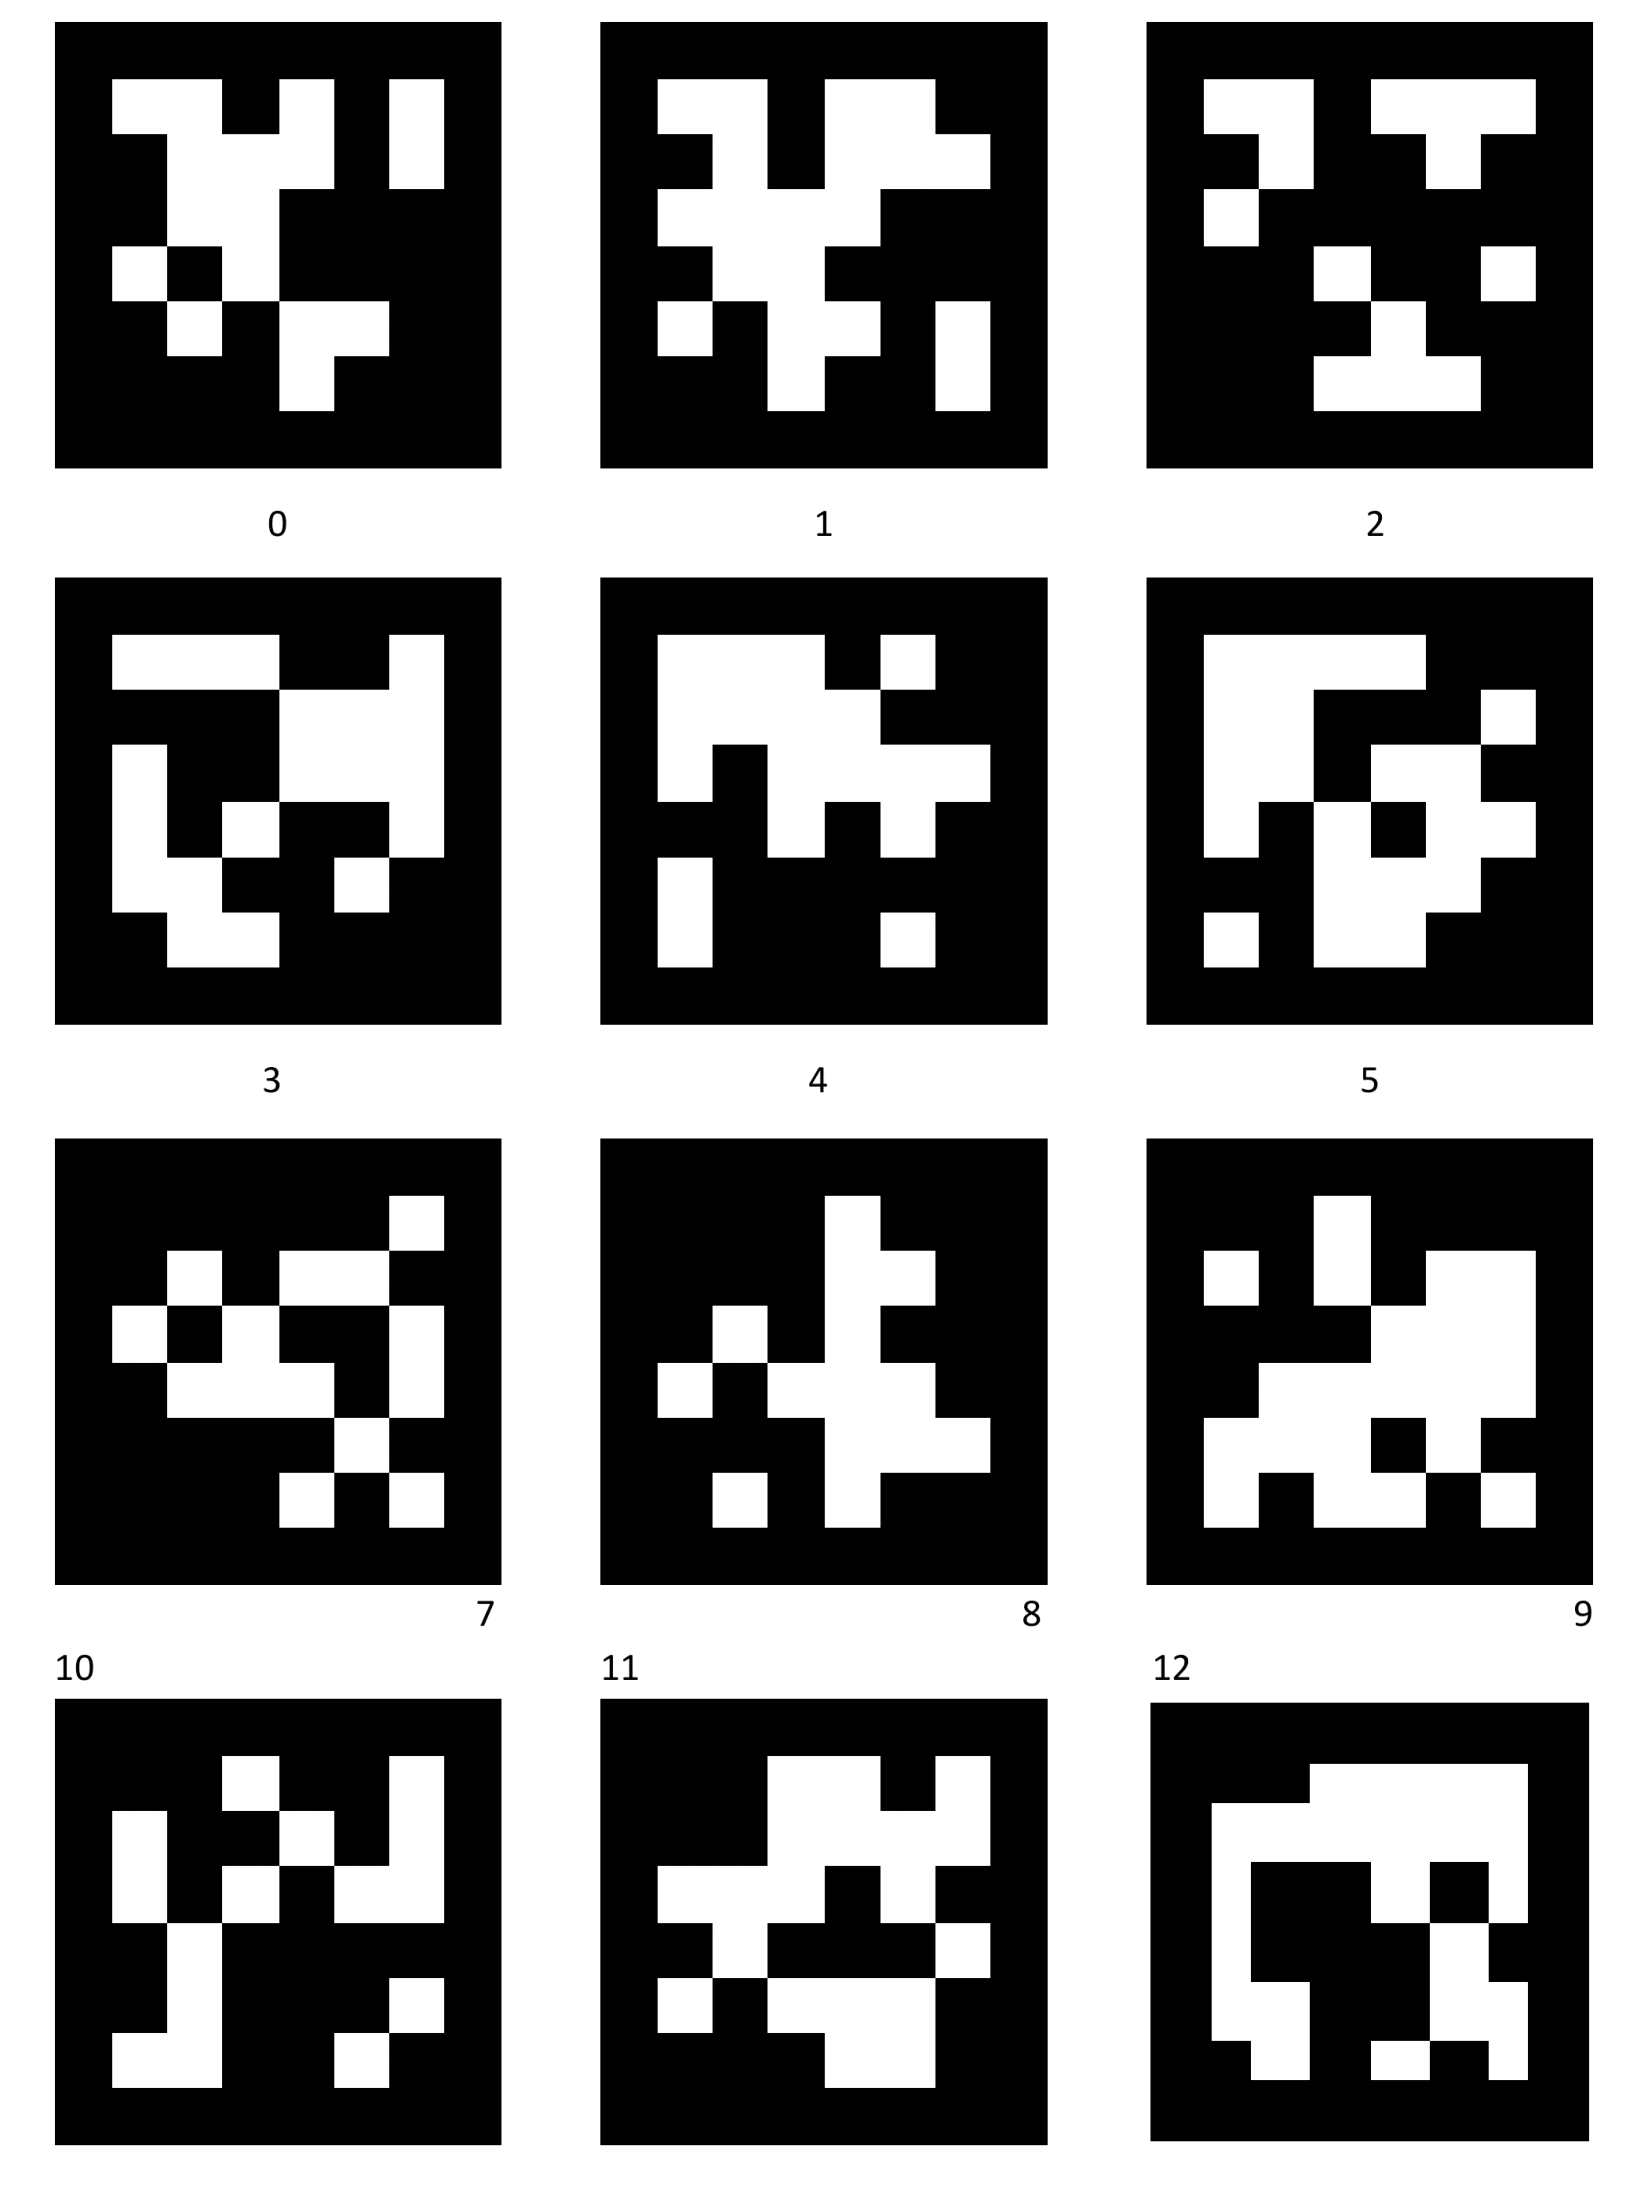
\includegraphics[width=.2\textwidth]{graphics/aptags.png}
    \caption{The apriltags board used for the stereopair calibration}
    \label{fig:aptags}
\end{figure}

Stereo pair calibration is a process of estimating the essential matrix $\mat{E}$ for a camera pair, which also can be computed from a relative rotation matrix $\mat{R}_{21}$ and a relative translation vector $\vec{t}_{21}$ of a camera pair. 

There are multiple algorithms to do a stereo pair calibration.
Usually, a calibration chessboard is used (\autoref{fig:chb}) for a standard stereo camera with parallel or converging optical rays.
It can be detected and used only when the whole chessboard is seen in both images.
It is a disadvantage for cameras with a small overlapping zone and diverging optical rays, only if a really big chessboard is used at a considerable distance.
For this reason, it is better to use some other pattern, for example, a set of apriltags \cite{Malyuta2019} which can be detected separately. 

\subsection{Least-square estimation of transformation}
\label{sec:lsq_umeyama}
The first approach assumes that cameras' poses are pre-measured, and the only necessary step is to correct one camera pose with respect to another.
Firstly it detects apriltag's from \textit{im1} and \textit{im2}, compute their 3D poses.
Then, estimate transformation parameters between two point sets, and find the correction transformation $\mat{T}_{correction}$.
The last step is to apply $\mat{T}_{correction}$ to $\mat{R}_{21}$ and $\vec{t}_{21}$ and obtain a corrected pose of the second camera.

\subsection{PnP-based algorithm}
\label{sec:pnp}
Another, a more general approach is based on solving a Perspective-n-Point (PnP) problem.
PnP is the problem of estimating a camera pose (translation and rotation) given a known set of 3D points and respective 2D projections from calibrated camera
\begin{equation}
    \lambda_i \begin{bmatrix} \vec{m}_i \\ 1 \end{bmatrix} = \mat{K} \mat{R} (\vec{X}_i - \vec{C}), \;\; i = \{0..n\}.
\end{equation}
No initial pose estimation is needed for this algorithm, but it can accelerate the solver if there is one.

\begin{figure}[h]
    \centering
    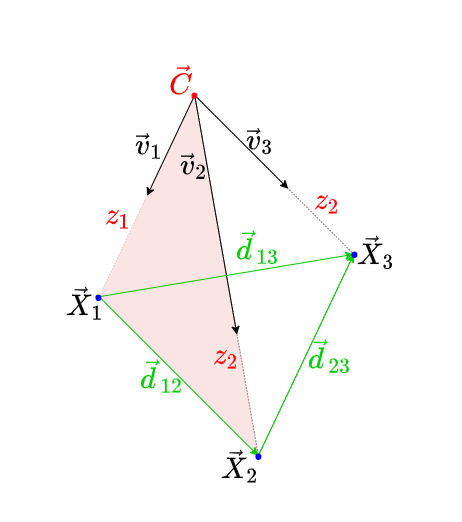
\includegraphics[width=.3\textwidth]{graphics/p3p.png}
    \caption{The P3P algotrithm visualization}
    \label{fig:p3p}
\end{figure}

The situation when $n=3$ is the minimal amount of points to solve the PnP problem, this method is called P3P.  
Firstly, let us define $\vec{v}_i = \mat{K}^{-1}\begin{bmatrix}\vec{m}_i \\ 1 \end{bmatrix}$, $\vec{v}_i \in \mathbb{R}^3$ . Then
\begin{equation}
    \label{eq:p3p_gen}
    \lambda_i \vec{v}_i = \mat{R} (\vec{X}_i - \vec{C}).
\end{equation}
If there is no rotation, the situation will look like on a figure \autoref{fig:p3p} where vectors $\vec{d}_i$ are known, so there is a system of three equations with three unknowns (vector $\vec{C}$).
If there is a rotation, firstly it can be elliminated by defining $z_i$ As
\begin{equation}
    \label{eq:p3p_rot}
    |\lambda_i| \cdot ||\vec{v}_i|| = || \vec{X}_i - \vec{C} || = z_i.
\end{equation}
Considering only angles between $\vec{v}_i$ and apply the cosine law per triangle ($\vec{C}$, $\vec{X}_i$, $\vec{X}_j$), $i, j = 1, 2, 3, i \neq j$
\begin{equation}
    ||\vec{d}_{ij}|| = z_i^2 + z_j^2 - 2z_iz_jc_{ij},
\end{equation}
where $||\vec{d}_{ij}|| = || \vec{X}_j - \vec{X}_i ||$, $c_{ij} = \cos(\angle \vec{v}_i \vec{v}_j)$.
After solving the system of three equations with three unknown $z_i$, there will be 4 sollutions including unreal, that should be verified on additional points \cite{Fischler1981}.
Having this, $\vec{C}$ can be found by trilateration (3 sphere intersection) from $\vec{X}_i$ and $z_i$; then $\lambda_i$ from \eqref{eq:p3p_rot} and $\mat{R}$ from \eqref{eq:p3p_gen}.
% \subsection{}
% It is also possible to calibrate with correctly matched correspondences only, but the precision can worsen.
% Having two calibrated cameras, it is possible to compute essential matrix $\mat{E}$ \autoref{eq:E} from at least 5 corresponding points, and then decompose it to $\mat{R}_{21}$ and $\vec{t}_{21}$.

\section{Features extraction, matching and filtering}
\label{sec:features}
In a computer vision, \textit{features} are representations of unique pieces of information from the image scene, such as points, edges and objects.
A feature detector is an algorithm for extracting features from an image.
There are multiple of them, but in this solution, ORB \cite{Rublee2011} is used. 
This algorithm claims to be of the same accuracy as the state-of-the-art SIFT detector but a few times faster. 

The next important part is a feature matcher. 
After keypoints with descriptors are detected on both images, the matcher should match them between each other, to create correspondences.
It can be done by bruteforce comparison of descriptors, nearest neighbors approximation or even using neural networks.

\section{Features pose estimation}

3D scene points' poses can be computed by having pairs of correspondent points taken by calibrated cameras.
This process is called triangulation.

\subsection{Shortest distance}
One method to make a triangulation is to find the shortest distance between two rays.
According to epipolar geometry properties, \autoref{sec:epipolar_geometry}, vectors $\vec{d}_1$ and $\vec{d}_2$ \autoref{fig:epipolar_std} intersects at the 3D point $\vec{X}$.
However, in the real world, lines can be at some distance from each other, so $\vec{X}$ is the point closest to both lines.

It is possible to compute $\vec{d}_1$ and $\vec{d}_2$ in the common coordinate frame having cameras' poses and image features.
Then define two lines $d_1$ and $d_2$ in a vector form:
\begin{equation}
    d_1: p_1 = \vec{C}_1 + t \vec{d}_1,
\end{equation}
\begin{equation}
    d_2: p_2 = \vec{C}_2 + s \vec{d}_2,
\end{equation}
where $\vec{d}_1$ and $\vec{d}_2$ are directional vectors, $\vec{C}_1$ and $\vec{C}_2$ are 3D points located on respective lines, $s$ and $t$ are free parameters that uniquely define points $p_1$ and $p_2$. 
To minimize the distance between two lines, such $p_1$ and $p_2$ are needed that the line with directional vector $\vec{p_1p_2} = \vec{l}$ will be orthogonal to $d_1$ and $d_2$ which means
\begin{equation}
    \label{eq:ldd1}
    \vec{l} \cdot \vec{d}_1 = 0,
\end{equation}
\begin{equation}
    \label{eq:ldd2}
    \vec{l} \cdot \vec{d}_2 = 0.
\end{equation}
It is a system of two equations with two $s$ and $t$ unknown.
So after $s$ and $t$ are found, $\vec{X}$ can be compute as $\vec{X} = \frac{p_1 + p_2}{2}$.

\subsection{SVD Triangulation}
\label{sec:svdtriang}
Singular value decomposition (SVD) triangulation is another method that is more optimal and wide-used.
It computes 3D points from camera matrices $\mat{P}_1$, $\mat{P}_2$ and 2D correspondences. 
This method is described in \cite{hartley_zisserman_2004}.

The projection equation \eqref{eq:projection} can be rewritten as
\begin{equation}
    \lambda_i \begin{bmatrix} 
        u_i \\ v_i \\ 1 \end{bmatrix} = \mat{P}_i
    \begin{bmatrix} \vec{X} \\ 1
    \end{bmatrix},
\end{equation} 
where $\mat{P}_i$ decomposes as in \eqref{eq:p_general}, and $\lambda_i \neq 0$, i = \{1, 2\}.
After eliminating $\lambda_1$, $\lambda_2$, let $D$ be such matrix that
\begin{equation}
    \mat{D} \begin{bmatrix} \vec{X} \\ 1 \end{bmatrix} = \vec{0}, \;\;\;\;\;
    \mat{D} = \begin{bmatrix}
        u_1 (p_1^3)^\top - (p_1^1)^\top \\
        v_1 (p_1^3)^\top - (p_1^2)^\top \\
        u_2 (p_2^3)^\top - (p_2^1)^\top \\
        v_2 (p_2^3)^\top - (p_2^2)^\top \\
    \end{bmatrix}, \;\;\;\;\; \mat{D} \in \mathbb{R}^{4, 4}.
\end{equation}

The solution is $u_4$, the last column of the $\mat{U}$ matrix from $\mathsf{SVD}(\mat{D}^\top \mat{D}) = \mat{U}, \mat{S}, \mat{V}^\top$.



